%%%%%%%%%%%%%%%%%%%%%%%%%%%%%%%%%%%%%%%%%%%%%%%%%%%%%%%%%%%%%%%%%%%%%%%%%%%%%%%%%%%%%%%%%%%%%%%%%%%%%%%
% Sablona pro projekty ekonometrickych predmetu                                                     %%%
% Vytvoreno v ramci grantu: Ekonometricke nastroje a techniky v realnych ekonomickych aplikacich    %%%
% Autor: Jakub Bucek (jakubbucek@mail.muni.cz)                                                      %%%
% Pripominky, dotazy, namety smerujte na autora nebo na Daniela Nemce (danek@mail.muni.cz)		    %%%
% Vytvoreno: 1.12.2014                                                                              %%%
%%%%%%%%%%%%%%%%%%%%%%%%%%%%%%%%%%%%%%%%%%%%%%%%%%%%%%%%%%%%%%%%%%%%%%%%%%%%%%%%%%%%%%%%%%%%%%%%%%%%%%%

\documentclass[12pt,a4paper,oneside,final]{article}

%%%%%%%%%%%%%%%%%%%%%%%%%%%%%%%%%%%%%%%%%%%%%%%%%%%%%%%%%%%%%%%%%%%%%%%%%%%%%%%%%%%%%%%%%%%%%%%%%%%%%%%
%%%%%%%%%%%%%%%%%%%%%%%%%%%%%%%%%%%%%% ZAKLADNI NASTAVENI %%%%%%%%%%%%%%%%%%%%%%%%%%%%%%%%%%%%%%%%%%%%%

%% Nastaveni kodovani
\usepackage[utf8]{inputenc} 
\usepackage[IL2]{fontenc} %% fonty vhodne pro sazbu ceskych a slovenskych dokumentu
\usepackage[slovak]{babel}

\usepackage{subcaption}
%\usepackage{subfig}

%% Fonty
\usepackage{mathptmx}  %% volne dostupny font Adobe Times Roman
% \usepackage{bookman}
% \usepackage{charter}
% \usepackage{fourier}
% \usepackage{mathpazo}
% \usepackage{newcent}
% \usepackage{palatino}
% \usepackage{utopia}

%% Baliky potrebne pro sazbu matematiky
\usepackage{amssymb,amsthm,amsmath}
\usepackage{bm}
\usepackage{tabularx} %% vylepsene tabulky

%% Balik nutny pro sablonu
\usepackage{garfield} %% nacteni stylu sablony

%% Vlastní definice
\renewcommand\vec[1]{\ensuremath\boldsymbol{#1}} %% tucne vektory
\newtheorem{veta}{Věta}[section]
\swapnumbers
\theoremstyle{definition}
\newtheorem{definice}{Definice}
\theoremstyle{remark}
\newtheorem*{pozn}{Poznámka}
\numberwithin{equation}{section}

%%%%%%%%%%%%%%%%%%%%%%%%%%%%%%%%%%%%%%%%%%%%%%%%%%%%%%%%%%%%%%%%%%%%%%%%%%%%%%%%%%%%%%%%%%%%%%%%%%%%%%%
%%%%%%%%%%%%%%%%%%%%%%%%%%%%%%%%%%%%%%%% TITULNI STRANA %%%%%%%%%%%%%%%%%%%%%%%%%%%%%%%%%%%%%%%%%%%%%%%

\NazevPrace{Modelovanie časových radov z monitorovacieho systému Hawkular}
\Autor{Bc. Pavol Loffay}
\Univerzita{Masarykova univerzita}
\Fakulta{Fakulta informatiky}
\Obor{Service Science Management Engineering}
\Mail{p.loffay@mail.muni.cz}
\DatumOdevzdani{\today}
\Abstrakt{
 Práca spracováva predikciu časových radov prevziatych z monitorovacieho systému
 Hawkular\footnote{Dostupné na \url{http://www.hawkular.org}}. Tento systém dokáže
 monitorovať Java aplikácie, alebo fyzický hardvér na ktom je spustený.
 Z množiny pozorovaných metrík boli vybraté následujúce: vyťaženie Java hromady (heap),
 miesto na disku a počet voľných databázových spojení. Tieto časové rady som analyzoval
 a cieľom bolo zostaviť model, ktorý nejlepšie popisoval priebeh danej časovej rady. 
 V práci som postupoval podľa Box\,--\,Jenkinsovej metodológie.
}
\KlicovaSlova{Časová rada; ARIMA; Hawkular; ACF}
\JELklasifikace{C53}

%%%%%%%%%%%%%%%%%%%%%%%%%%%%%%%%%%%%%%%%%%%%%%%%%%%%%%%%%%%%%%%%%%%%%%%%%%%%%%%%%%%%%%%%%%%%%%%%%%%%%%%
%%%%%%%%%%%%%%%%%%%%%%%%%%%%%%%%%%%%%% ZACATEK DOKUMENTU %%%%%%%%%%%%%%%%%%%%%%%%%%%%%%%%%%%%%%%%%%%%%%

\begin{document}
\VytvorTitulniStranu

\section{Úvod}
Monitorovanie doležitých business aplikácii, ako sú napríklad bankové systémi alebo rôzne
servery na ktorých bežia služby ktoré sú využívané 24/7 je veľmi dôležité. Vačšina
monitorovacích systémov dokáže upozorniť administrátora na vyťaženie pri prekročení
hraničnej hodnoty. V monitorovacom systéme Hawkular je možné zapnúť predikciu, takže
administrátor bude upozornený vopred ak by náhodov malo dôjsť k prekročeniu spomenutej
hraničnej hodnoty. Použíté modely časových rád v systéme Hawkular sú varianty
exponenciálneho vyrovnania. Modely ARIMA nemohli byť použité z dôvodu nestacionarity dát 
a náročnosti na výpočet\,--\,systém je schopný analyzovať aj niekoľko tisíc model naraz. 

V tejto práci sa zameriam na konštrukciu optimálneho ARIMA modelu, ktorý následne porovnám
s exponenciálnym vyrovnaním konkrétne Holtovou metódou s linárnym trendom.

\section{Analýza Java Heap metriky}
V tejto kapitole budeme analyzovať časovú radu, ktorá popisuje vyťaženosť Java heap-u v
čase.

Graf časovej rady:
\begin{figure}[htb] \centering
    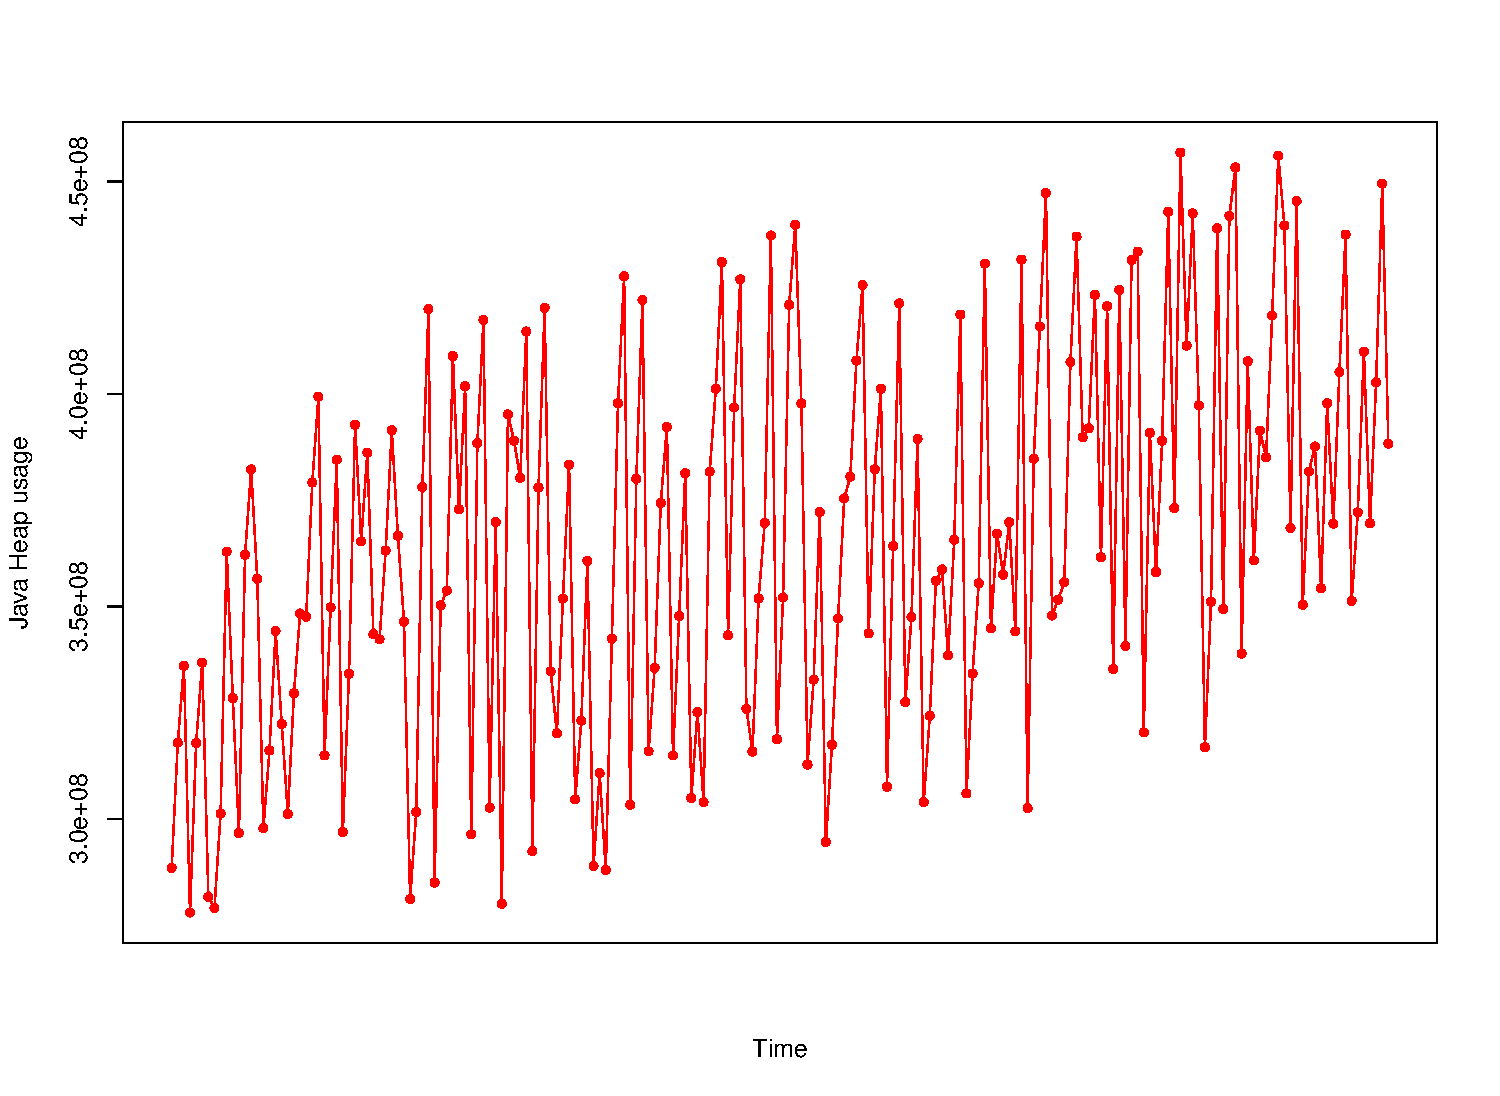
\includegraphics[width=.8\textwidth]{images/heap_series.pdf}
    \caption{Vyťaženosť Java Heap-u v čase.}
    \label{obr:heap} % unikatni navesti, pomoci ktereho se budeme v textu odvolavat na dany obrazek
\end{figure}

\subsection{Identifikácia ARIMA modelu}
Z obrázka \ref{obr:heap} je možné usúdiť, že časová rada obsahuje mierny lineárny trend,
čo by znamenalo že je nestacionárna. Následne si vykresíme autokorelačnú (zkrátene) a
parciálknu autokorelačnú funkciu (zkrátene PACF).

\begin{figure}[!tbo] \centering
    \begin{subfigure}[b]{0.45\textwidth}
        \centering
        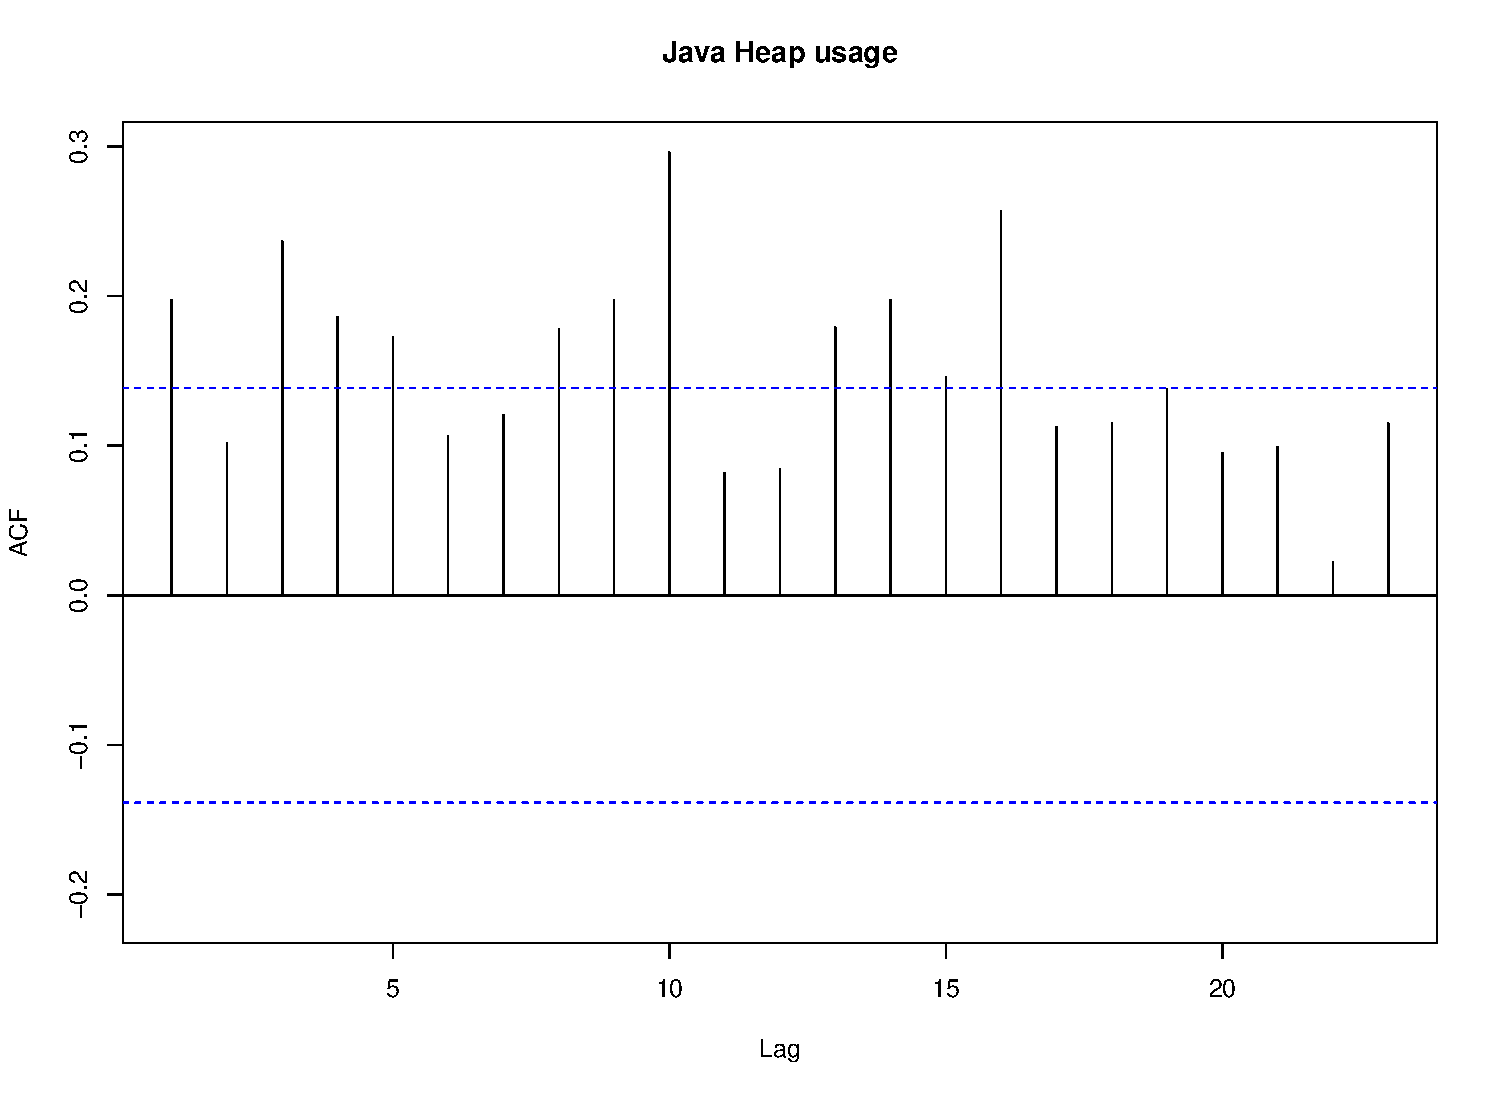
\includegraphics[width=1\linewidth]{images/heap_acf.pdf}
        \caption{Autokorelačná funkcia.}
        \label{obr:heap_acf}
    \end{subfigure}
    \begin{subfigure}[b]{0.45\textwidth}
        \centering
        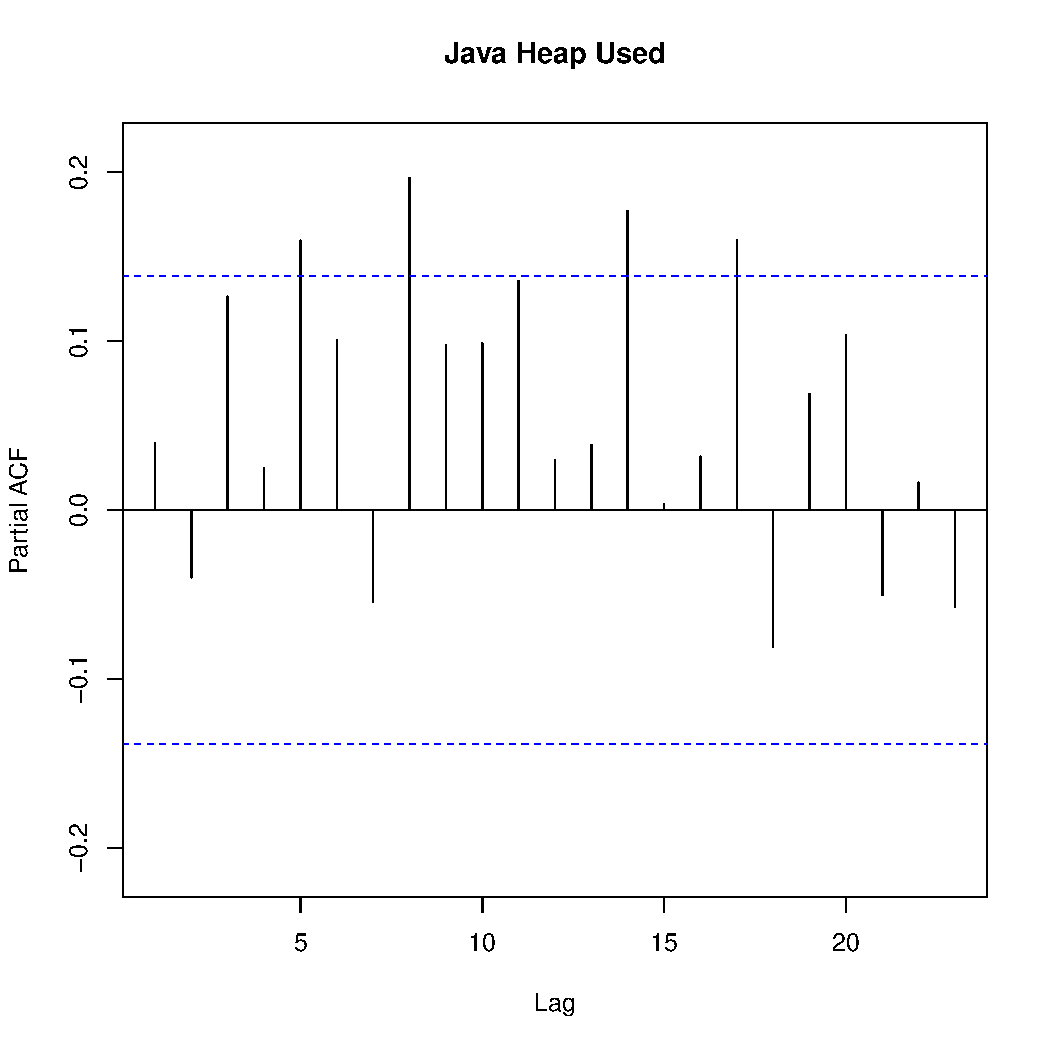
\includegraphics[width=1\linewidth]{images/heap_pacf.pdf}
        \caption{Parciálna autokorelačná funkcia.}
        \label{obr:heap_pacf}
    \end{subfigure}
%    \caption{Parciálna autokorelačná funkcia.}
    \label{fig:test}
\end{figure}

Z obrázka \ref{obr:heap_acf} je vidieť že hodnoty ACF sú kladné ale avšak relatívne blízke
nule, stým že významne neklesajú k nule. 
V grafe ACF \ref{obr:heap_acf} taktiež nie sú prítomné prítomné periodicky posunuté vysoké hodnoty, 
takže rada neobsahuje sezónnosť.

Keďže hodnotz ACF so zvyšujúcim spozdením neklesali k nule rozhodli sme sa urobiť ADF test
na test stacionarity.

\begin{minipage}{\linewidth}
\begingroup
\fontsize{9pt}{7pt}\selectfont
\begin{verbatim}
> adfTest(as.numeric(b$avg), lags = 0, type="nc")
Title:
 Augmented Dickey-Fuller Test
Test Results:
  PARAMETER:
    Lag Order: 0
  STATISTIC:
    Dickey-Fuller: -0.976
  P VALUE:
    0.3042 
\end{verbatim}
\endgroup
\end{minipage}

Z vyšie uvedeného ADF testu môžeme vidieť, že nulovú hypotézu časová rada
nie je stacionárna by sme na hladine významnosti 0.05 ne zametli. Takže naša časová rada
je nestacionárna. Pre overenie skusíme KPSS test, ktorého nulová hypotéza je že časová 
rada je stacionárna.

\begin{minipage}{\linewidth}
\begingroup
\fontsize{9pt}{7pt}\selectfont
\begin{verbatim}
> kpss.test(as.numeric(b$avg))
	KPSS Test for Level Stationarity
data:  as.numeric(b$avg)
KPSS Level = 2.5916, Truncation lag parameter = 3, p-value = 0.01
\end{verbatim}
\endgroup
\end{minipage}
Na hladine významnosti by sme nulovú hypotézu zamietli. Oba testy nám ukázali, že časová
rada nie je stacinárna. 
Následne môžeme pomocou KPSS testu testovať, či je daná časová rada trend stacinárna:
\begin{minipage}{\linewidth}
\begingroup
\fontsize{9pt}{7pt}\selectfont
\begin{verbatim}
> kpss.test(as.numeric(b$avg), null='Trend')
	KPSS Test for Trend Stationarity
data:  as.numeric(b$avg)
KPSS Trend = 0.073128, Truncation lag parameter = 3, p-value = 0.1

> ndiffs(as.numeric(b$avg))
[1] 1

> diff = diff(as.numeric(b$avg))
\end{verbatim}
\endgroup
\end{minipage}
Z výstupu je jasné, že rada je trend stacinárna takže nulovú hypotézu na hladine 0.05
nezamietame.

Ďalej pokračujeme vykreslením ACF a PAC. Z obrázka parciálnej autokorelačnej funkcie \ref{heap_diff_pacf} 
možme usúdiť, že do úvahy by spadal model \emph{AR(15)} alebo \emph{MA(1)}. Keďže ACF je
možné obmedziť krivkou U, tak je lepšie vybrať model \emph{MA(1)} \cite{cipra}.
\begin{figure}[!tbo] \centering
    \begin{subfigure}[b]{0.45\textwidth}
        \centering
        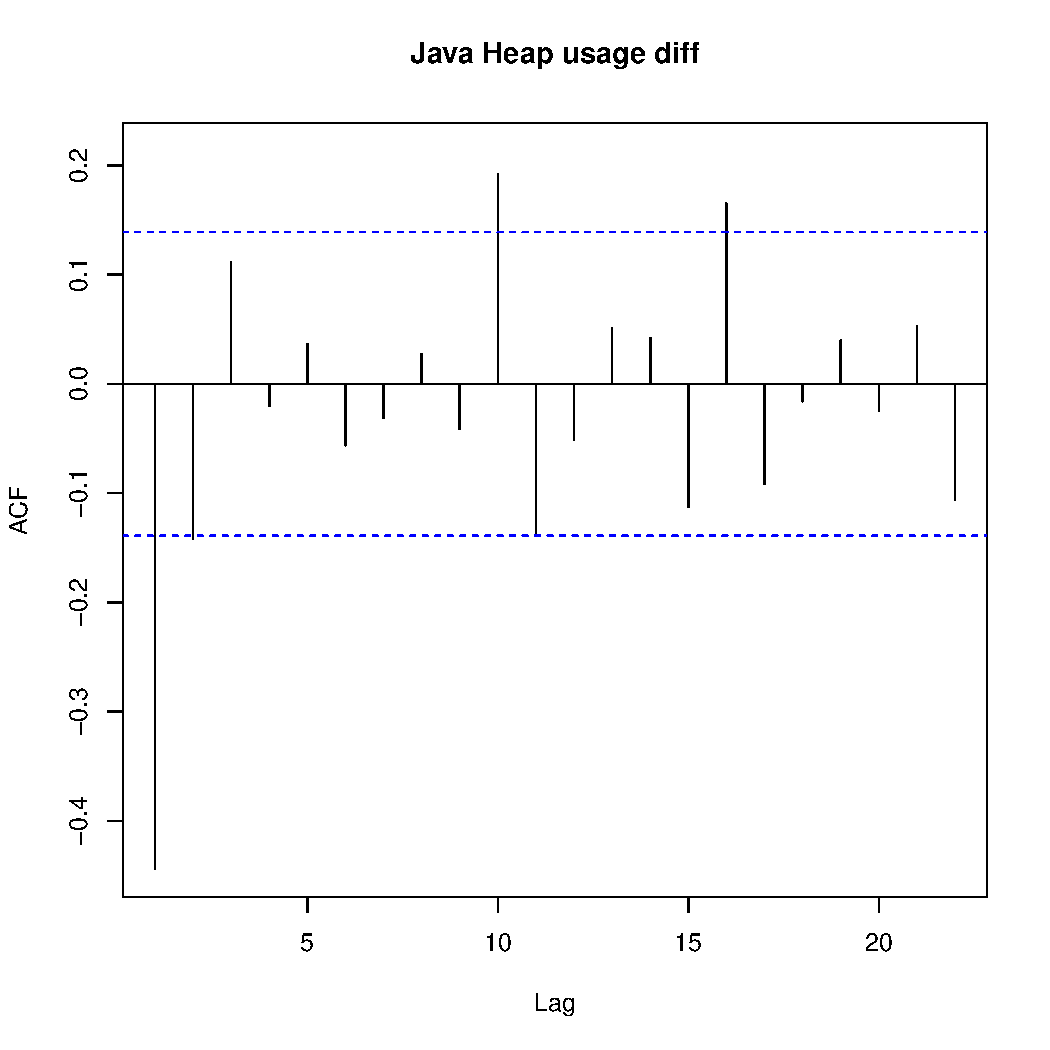
\includegraphics[width=1\linewidth]{images/heap_diff_acf.pdf}
%        \caption{Autokorelačná funkcia rady.}
        \label{obr:heap_diff_acf}
        %Pcf(diff, main='Java Heap usage diff')
    \end{subfigure}
    \begin{subfigure}[b]{0.45\textwidth}
        \centering
        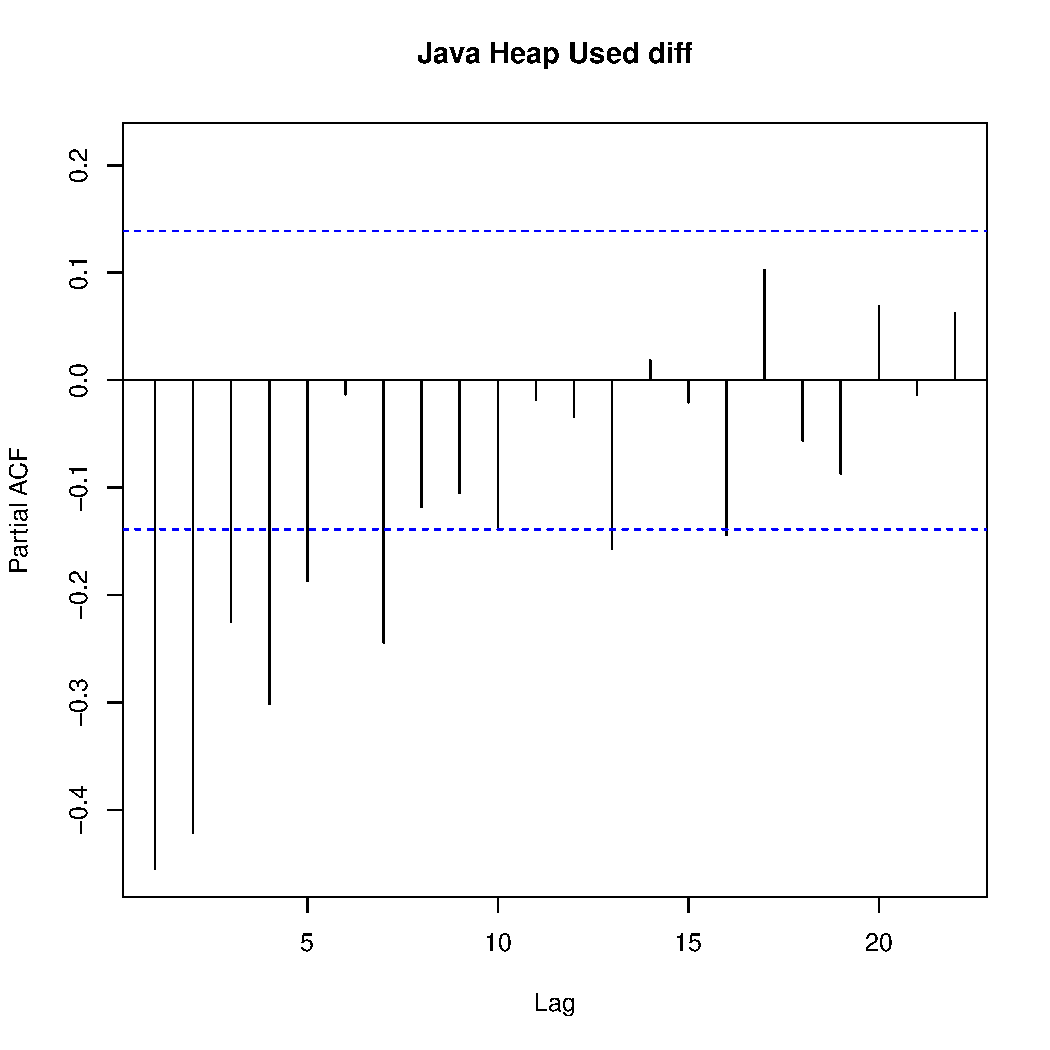
\includegraphics[width=1\linewidth]{images/heap_diff_pacf.pdf}
%        \caption{Parciálna autokorelačná funkcia rady.}
        \label{obr:heap_diff_pacf}
        %Pacf(diff, main='Java Heap usage diff')
    \end{subfigure}
    \caption{ACF a PACF diferencovanej časovej rady.}
    \label{fig:test}
\end{figure}

Alternatívny spôsob voľby modelu je pomocou informačných kritérii. Tento spôsob je
vhodný pre plne automatizované spracovanie \cite{cipra} napríklad v ekonometrických 
softvéroch. K identifikácia modelu ARMA(p, q) sa priktupuje ako k minimalizácii funkcie
\ref{rov:inf_k}

\begin{eqnarray} \label{rov:inf_k}
    (\hat{p}, \hat{q}) =arg\ \underset{(k,l)}{min}\ A(k, l)
\end{eqnarray}

\emph{A} je vhodné kritérium pre ktorého konštrukciu musíme odhadnúť model ARMA(k,l). Pri
minimalizácii postupujeme postupne inkrementujeme obidva parametre k, l.
V tejto práci sme zvolili Akaikeho informačné kritérium:

\begin{eqnarray} \label{rov:aic}
    A(k,l) = AIC(k,l) = ln\hat{\sigma}^{2}_{k,l} + \frac{2(k+l+1)}{n}
\end{eqnarray}

Ako je vidieť z \ref{rov:aic} kritérium prenalizuje veľké rády k a l. 
$\hat{\sigma}^{2}_{k,l}$ je smerodajná odchylka reziduí.

\section{Ekonomický model}

\section{Ekonometrický model}

\section{Odhadnutý model}

\section{Interpretace výsledků}

\section{Záver}
\cite{cipra}

\section*{Poďakovanie}
Na záver by som chcel poďakovať Ing. Danielovi Němcovi, Ph.D. za návrh na vypracovanie
tejto témi a za veľmi príjemné a užitočné konzultácie. Ďalej by som chcel poďakovať Ester
Železňákovej za gramatickú korektúru textu.

\bibliographystyle{czechiso}
\bibliography{bibliography}

%% Pokud nechcete pouzit prilohy, muzete nasledujici radky az po \end{document} smazat
\newpage
\renewcommand{\thesection}{\Alph{section}}
\setcounter{section}{0}
\renewcommand{\thepage}{\roman{page}}
\setcounter{page}{1}

\section{Prílohy}
\label{priloha}

\end{document}

